\documentclass[../report.tex]{subfiles}
\begin{document}
\chapter{Literature Study}
\label{ch:literature_study}

\newfontfamily\myfont{Times new roman}

The thesis project commences with a study of literature, this is intended to introduce the main concepts that will be used as the foundation of the methodologies used, as well as supplement the discussion of any results gathered. Literature studies are conducted in fields related to the research project, thus the first field to be surveyed will be that of Reinforcement Learning, and the second field to be surveyed is the developments of the Flying-V. 


\section{Reinforcement Learning Foundations}

The basic idea of reinforcement learning is to have some agent associate rewards with actions that help realize a goal and promote the agent to take more of such actions by asking it to maximize the reward. The agent is not told what the goal is explicitly, its' only interface with the world around it is through executing these actions, and observing that it has transitioned into some state and received some reward. Reinforcement learning can be thought of as a way in which theorists have attempted to codify and formulate algorithms for, the universal experience of learning through trial and error. Much like how a child learns to walk, or a dog learns to sit, it is through reinforcement learning that machines can learn how to perform tasks that might not be easily programmed. Through this codification, computer programs have been made that demonstrated impressive levels of learning; for example, programs can learn through reinforcement learning to play various high-dimensional board games to a level of expertise surpassing any living player \cite{alpha_zero}, and a robotic arm can learn hand dexterity and mimic the hand movements of a human \cite{OpenAI_dexterity}.

Understanding how the reinforcement learning algorithms work behind such examples and how they may be applied to flight control will require understanding the foundations first, thus this section will introduce the basic terminologies and ideas used to build these algorithms.


\subsection{Markov Decision Process}

The Markov decision process is the mathematical framework that is used to model sequential decision processes such as how an agent interacts with an environment, and it is what contextualizes all the ideas in reinforcement learning, for instance, the basic notion that an agent performs an action and receives a reward.

In such a framework, there exist two entities: the agent and the environment, and information flows from one entity to another to model making decisions and their resulting consequences. In reinforcement learning the agent is sometimes also called the learner, it selects an action $A_t$ which gets fed to the environment, and the environment will provide the corresponding state $S_{t+1}$ which the agent has transitioned to as a result of action $A_t$ and the reward associated to that state transition $R_{t+1}$, the agent can subsequently use $S_{t+1}$ and $R_{t+1}$ to decide on the next time step's action $A_{t+1}$. A graphical depiction of this agent-environment interface in the Markov decision process is shown in \autoref{fig:mdp}.

\begin{figure}[H]
    \centering
    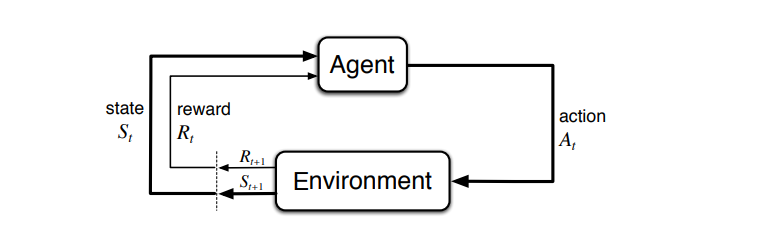
\includegraphics[width=\textwidth]{figures/01/mdp.png}
    \caption{Flow diagram of the agent-environment interaction central to the Markov decision process}
    \label{fig:mdp}
\end{figure}

This time trace of an agent-environment interaction is recorded in a so-called \textit{trajectory} $\mathcal{T}$, which is a chain of state-action-reward for the entire duration of the decision process written in the form expressed in \autoref{eq:trajectory}.

\begin{equation} \label{eq:trajectory}
    \mathcal{T} = S_{0}, A_{0}, R_{1}, S_{1}, A_{1}, R_{2}, \dots, S_{T-1}, A_{T-1}, R_{T}, S_{T}, A_{T}
\end{equation}


One central component of Markov decision processes is the dynamics of the environment. In the simpler case of finite and discrete processes, the dynamics of the environment can be considered to be a discrete conditional probability distribution $p(s', r|s,a)$ as shown in \autoref{eq:mdp_dynamics}. which returns the probability of transitioning to a state $s'$ and obtaining a reward $r$ given that the agent observed a previous state $s$ and executed an action $a$.

\begin{equation} \label{eq:mdp_dynamics}
    p(s', r|s,a) \doteq Pr\{St=s', R_t=r|S_{t-1}=a,A_{t-1} =a\}
\end{equation}

From \autoref{eq:mdp_dynamics}, it is possible to compute the expected reward for any state-action pairs $r(s,a)$:

\begin{equation}
    r(s,a) \doteq \mathbb{E}\{R_t | S_{t-1}=s, A_{T-1}=a\} = \sum\limits_{r}r\sum\limits_{s'}p(s', r|s,a)
\end{equation}

Modeling the environment dynamics, also referred to as modeling the Markov decision process dynamics, can also be done using other modeling methods. For example, state space systems of equations are commonly used when creating control systems, and as such are also used to serve as the dynamics model in the Markov decision processes \cite{ss_example_1, ss_example_2, ss_example_3}. In both cases, one important property that the models possess is the \textit{Markov property}, also referred to as the memoryless property. This property states that to predict the system in the next time step, only information from the current or time step before is necessary, which means that having any information from previous time steps does not influence the outcome of the prediction. This property is captured in \autoref{eq:markov_property}.

\begin{equation} \label{eq:markov_property}
    Pr\{St, R_t|S_{t-1},A_{t-1}\} = Pr\{St, R_t|S_1, \dots, S_{t-1}, A_1, \dots, A_{t-1}\}
\end{equation}


In reinforcement learning, having the dynamics of the environment possess the Markov property is useful as many algorithms assume that the evolution of the system can be perfectly predicted by only using information from the current time step \cite{markov_property}, which should be sufficient for a learner to decide what actions to take in order to enter into a trajectory which maximizes its' rewards.

In the context of flight control, the Markov decision process can be conveniently formulated using state space systems. For example, the action, state, and reward in \autoref{fig:mdp} can be considered equivalent to the control vector, the state vector, and an output vector in the state space formulation respectively. 

\subsection{Environment}

\subsection{Rewards and Returns}

The way in which learners in a reinforcement learning problem gauge their performance is through reward signals, this reward signal is made to be representative of the goal of the reinforcement learning problem.

Reward signals are central to the \textit{reinforcement} in reinforcement learning, as they are made to be associated with states and actions that get the agent closer to the goal, thus incentivizing the learner to repeat more of such actions with the ultimate effect of the agent becoming more proficient in the posed task. Strong parallels can be drawn between an agent in the reinforcement learning context becoming better at obtaining higher reward signals, and that of animal behavior adapting to receive more desirable stimuli in the context of domestic animal training, a so-called "Law of Effect"\cite{law_of_effect}. This parallel arises from the strong connections between reinforcement learning as a computer science and mathematical theory, and reinforcement learning as a field of psychology, and shows how ideas in reinforcement learning are often grounded in ideas from nature. 

In reinforcement learning nomenclature, a distinction in terminology exists between the reward being received every time step, and the cumulative reward that an agent receives over many time steps. While rewards are received every time step, when they are summed up over time, they are then referred to as the \textit{return}. For example, an episodic return refers to how much cumulative reward an agent has received throughout an episode. Formally, returns are defined by \autoref{eq:return} as the sum of all future discounted rewards, where the discount factor $\gamma \in [0,1]$ is introduced which allows for returns to be computed even when a task is not episodic but continuing, i.e. $T=\infty$. Increasing $\gamma$ from 0 to 1 increases the weight of rewards received later in time, which makes the agent more ``far-sighted", the opposite case of decreasing $\gamma$ causes the agent to be more ``myopic".

\begin{equation}\label{eq:return}
    G_t \doteq R_{t+1} + \gamma R_{t+2} + \dots + \gamma^{T-t-1}R_T = \sum\limits_{k=t+1}^T \gamma^{k-t-1} R_k
\end{equation}

The goal of a learner in reinforcement learning is to maximize the return $G_t$, this return can also serve as a convenient metric to evaluate the relative performance of agents.

\subsection{Policy}

A policy is what an agent follows to decide on what action to choose. Formally, a policy $\pi$ is defined as a functional mapping from state $s$ to the probability of choosing an action $a$, i.e. probability of action $a$ conditioned on state $s$:

\begin{equation}
    \pi(a|s) \doteq Pr\{A_t=a | S_t=s\}
\end{equation}

The specific formulation of $\pi(a|s)$ differs greatly from algorithm to algorithm, in fact, there is no restriction on the form of the probability distribution that $\pi(a|s)$ takes. For instance, it is permissible that $\pi(a|s)$ is deterministic, i.e. if the state is $s_1$, then action is $a_1$. The overarching theme is that an agent should follow a policy that will maximize its returns.

\subsection{Value Function}

Value functions predict how much return an agent will receive in expectation if it were to follow a policy $\pi$. Two types of value functions are commonly used in reinforcement learning, the state-value function $V_{\pi}(s)$ and the action-value function $Q_{\pi}(s, a)$. The state-value function is the expected return from being in any single state, mathematically this is defined as:

\begin{equation}\label{eq:state_value_function}
    v_{\pi}(s) \doteq \mathbb{E}_{\pi}\{G_t | S_t = s\}
\end{equation}

Where $V_{\pi}(s)$ is the value of state $s$, and $G_t$ is the return from time $t$ onwards when following the policy $\pi$. Notation of the expectation operator is slightly abused to include the $\pi$ to indicate that the agent is following policy $\pi$. The state-value function can be intuitively understood as how worthwhile it is to be in a certain state. The action-value function is defined as the expected return of a particular state-action pair, this can again be mathematically stated as follows:

\begin{equation}\label{eq:action_value_function}
    q_{\pi}(s, a) \doteq \mathbb{E}_{\pi}\{G_t | S_t = s, A_t = a\}
\end{equation}

Where $Q_{\pi}(s, a)$ is the value of taking action $a$ in state $s$, and $G_t$ is the return from time $t$ onwards when following the policy $\pi$. The action-value function can be intuitively understood as how worthwhile it is to take a certain action in a certain state.


\subsection{Bellman Equation}
The equation commonly referred to as \textit{the} Bellman equation is the Bellman equation for the state-value function, presented in \autoref{eq:state_bellman}, which is derived starting from the definition of the state-value function \autoref{eq:state_value_function}:

\begin{align*}
    v_{\pi}(s) &\doteq \mathbb{E}_{\pi}\{G_t | S_t = s\} \\
    &= \mathbb{E}_{\pi}\{R_{t+1} + \gamma G_{t+1} | S_t = s\}\\
    &= \sum\limits_{r, g_{t+1}}p(r,g_{t+1}|s)[r + \gamma g_{t+1}]\\
    &= \sum\limits_{a, s'}\sum\limits_{r, g_{t+1}}p(a, s', r, g_{t+1}|s)[r + \gamma g_{t+1}]\\
    &= \sum\limits_{a}\sum\limits_{s',r}\sum\limits_{g_{t+1}}\underbrace{p(a|s)}_{= \pi(a|s)}p(s',r|s,a)\underbrace{p(g_{t+1}|s', r, s, a)}_{= p(g_{t+1}|s') \text{, Markov}}[r + \gamma g_{t+1}]\\
    &= \sum\limits_{a}\pi(a|s)\sum\limits_{s',r}p(s',r|s,a)[r + \gamma \sum\limits_{g_{t+1}}p(g_{t+1}|s')g_{t+1}]\\
    &= \sum\limits_{a}\pi(a|s) \sum\limits_{s', r} p(s', r|s, a)[r + \gamma v_{\pi}(s')] \stepcounter{equation}\tag{\theequation}\label{eq:state_bellman}\\
\end{align*}

This equation defines an analytical relationship between the value function of successive states, suggesting that the value of a previous state can be calculated once the subsequent state's value function, the environment dynamics, and the followed policy are known.

Notice that the value function in \autoref{eq:state_bellman} is recursively defined. This recursive formulation lends itself readily to dynamic programming techniques, which simply means that \autoref{eq:state_bellman} is adopted as an update equation for estimates of the state value function, where by iteratively applying this update the estimate converges towards the true value. The Bellman equation of \autoref{eq:state_bellman} was first derived by Richard Bellman and is associated with the basic foundations of the field of dynamic programming \cite{dp}.

There also exists a Bellman equation for the action-value function, which is presented in \autoref{eq:action_bellman}.

\begin{equation}\label{eq:action_bellman}
    q_{\pi}(s,a) \doteq \sum\limits_{s', r} p(s', r|s, a)[r + \gamma v_{\pi}(s')] 
\end{equation}

\section{Dynamic Programming}

One major direction of reinforcement learning research focuses on the use of \textit{Dynamic Programming} techniques, which has an emphasis on tackling optimal control problems using reinforcement learning\cite{rl_and_dp}. Dynamic programming is a term coined by Richard Bellman, it has roots in the field of optimization and is used to refer to the problem-solving approach of divide and conquer, where a more complicated problem is broken into sub-problems for which recursive algorithms can be devised to come up with their solutions\cite{dp}. In the context of reinforcement learning, classical applications of Dynamic programming revolved around the Bellman equation stated in \autoref{eq:state_bellman} and results in the method known as \textit{Policy Iteration}, which involved obtaining the optimal value function and policy for Markov decision problems which are \textit{finite}, which is to say that the state $s$ and action $a$ belong to countable sets that may be denoted $\mathcal{S}$ and $\mathcal{A}$ respectively.

\subsection{Policy Iteration}

This method iteratively applies two steps to find the optimal value function and policy, these steps are \textit{policy evaluation} and \textit{policy improvement}. The method can be outlined as follows:

\begin{enumerate}
    \item Initialize $\pi(a|s)$ and $V_{\pi'}(s)$ arbitrarily.
    \item Perform Policy Evaluation to compute the value function of $\pi$
    \item Perform Policy Improvement to find a more optimal policy 
    \item Repeat from Step 2 until $\pi$ and $v_{\pi}(s)$ have converged.
\end{enumerate}



\subsubsection{Policy Evaluation}

For a given policy $\pi$, the value function of this policy $v_{\pi}$ is computed by starting with an initial estimate $v_{\pi, 0}$ and recursively applying the Bellman equation on all $s$ as an update rule as shown in \autoref{eq:policy_eval}. This update will be applied until the value function has converged, where convergence can be defined in several ways, the simplest of which is when the norm of the difference between subsequent value functions is smaller than a small constant $\epsilon$.

\begin{equation}\label{eq:policy_eval}
    v_{\pi, k+1}= \sum\limits_{a}\pi(a|s) \sum\limits_{s', r} p(s', r|s, a)[r + \gamma v_{\pi, k}(s')] \quad \forall s \in \mathcal{S}
\end{equation}

Note that to compute the update formulated in \autoref{eq:policy_eval}, the environment dynamics $p(s',r|s,a)$ needs to be known and defined, which is an assumption made during the policy evaluation step.

By inspection of \autoref{eq:state_bellman}, it can be seen that the update equation \autoref{policy_eval} will only converge when the estimation $v_k$  is equl to the true value function of $\pi$.

\subsubsection{Policy Improvement}

For any given value function $v_{\pi}$, an improved policy $\pi'$ is obtained by making $\pi'$ deterministic and greedy with respect to $v_{\pi}$. This is done by defining $\pi'$ to choose the action that has the highest action value in each state $s$:

{\myfont
\begin{equation}\autoref{eq:policy_improvement}
    \pi'(a|s) = \begin{cases}
    1,& \text{if } a = \underset{a}{\text{argmax}} \ q_{\pi}(s,a) \\
    0,              & \text{otherwise}
\end{cases}
\end{equation}
}

The policy improvement step is guaranteed to find a policy that is at least as good as the previous policy, and in the case of a finite Markov decision process, the policy improvement step is guaranteed to find the optimal policy \cite{dp}.


\subsection{Adaptive Critic Design}

Finite Markov decision problems are characterized by their discrete and small number of states and actions that are possible


\section{Deep Reinforcement Learning}

\subsection{Temporal Difference Learning}

\subsection{Function Approximators and Deep Learning}

Deep learning refers to the subfield of machine learning which studies deep neural networks and their applications. This field has its origins in the ideas of artificial neural networks and is a scientific effort that has dramatically changed the idea of what an artificial neural network is and what it might be capable of. Deep neural networks fundamentally are an expansion of artificial neural networks, they use the same basic architecture of a neural network, with layers of interconnected neurons between a surface or input layer and a final output layer. The distinction between deep and artificial neural networks is that deep neural networks use many more layers and nodes than are typical in artificial networks,

\subsection{Merging TD \& Deep Learning}

Basic temporal difference algorithms utilize tabular look ups to retreive the value function of each state or state-action pair, this can hinder scaling to larger problem spaces which have many state or action variables, as the number of values to be stored increases combinatorially. The idea was thus put forth that function approximators should be used to approximate these look up tables which provided the scaling power necessary for higher dimensional tasks \cite{function_approximators}, with deep neural networks and multi layer perceptrons becoming popular approximators as they demonstrate a better scalability and approximation power \cite{drl_benchmarking, drl_atari, drl_humanlvl}. However, these function approximators need not necessarily be deep neural networks; in fact, early works focused on the application of simpler and smaller-scale approximations. Such as using coarse tile encoding, linear polynomials, Fourier basis, and many more.


\section{Classes of Reinforcement Learning Algorithms}

At the highest level, RL algos can be classified along three main dimensions:

\begin{itemize}
    \item model-based vs model-free
    \item policy-based vs value-based
    \item on-policy vs off-policy
\end{itemize}


\section{Synopsis}



\end{document}